\section{CNN accelerator overclocking} \label{sec:framework}
Overclocking can boost the clock frequency of CNN accelerators and is potentially beneficial to both 
the performance and energy efficiency. However, the timing violation may lead to distinct errors which 
may degrade the neural network prediction accuracy or even affect the functionality of the accelerators. 
In this section, we will explore the use of overclocking on FPGA based CNN accelerators to benefit from 
overclocking and minimize its negative influence.

\subsection{Overclocking overview}
Based on the intensity of overclocking and timing 
violation, we divide the overclocking incurred errors into different 
categories so that corresponding design methods can be used to 
alleviate the resulting problems efficiently. While it is difficult 
to precisely quantize the timing violations directly at runtime, we use 
the neural network prediction accuracy loss as the main 
classification metric. When there is only minor prediction accuracy 
loss which is less than 1\%, the penalty is usually acceptable 
and nothing needs to be done. 

When the prediction accuracy loss ranges from 1\% to 10\%, the accelerator 
still functions and the moderate accuracy loss can still be salvaged. 
As the neural network models are usually obtained 
from offline training on general purposed processors (GPPs) which assumes the 
neural networks to be executed on an equivalent computing device, 
the computing on overclocked CNN accelerator varies and does not match 
with the assumption. By getting rid of the computing difference between 
inference and training, the prediction accuracy can be improved.

When there are sever timing violations and 
the accuracy loss is over 10\%, there is usually little chance to recover 
without improving the timing and the status of the accelerator 
may not be steady. It may result in considerable computing errors 
and dramatic prediction accuracy loss 
or even system stall due to critical control signal errors.  

In addition, the timing errors incurred by overclocking are difficult 
to predict and there is no guarantee that the accelerator can function properly 
with just slightly overclocking. Typically, we expect that the lower overclocking setup 
may also lead to severe computing errors with lower probability.
Fig \ref{fig:loss-estimation} shows the possible accuracy loss status 
transition graph. It indicates that we should take the worst case 
into consideration even when the overclocking setup is relatively
conservative.

\begin{figure}
        \center{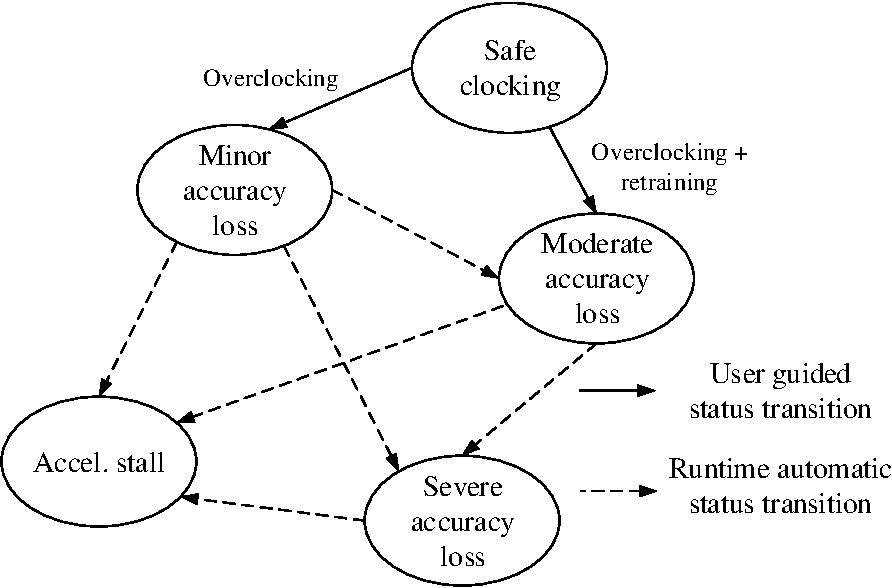
\includegraphics[width=0.75\linewidth]{status_transition}}
    \caption{Overclocked CNN accelerator status transition graph.}
\label{fig:loss-estimation}
\vspace{-1em}
\end{figure}

\subsection{Techniques for mitigating overclocking errors}
As discussed in the above section, there are different overclocking options and 
they have distinct influence on the neural network execution. Corresponding approaches 
will be detailed in this section to mitigate all the negative influence.

\subsubsection{Accuracy loss estimation}
Before we start to address the different overclocking problems, we need to 
determine the status of the overclocked CNN accelerator at runtime. 
Assume that the CNN accelerator performs inference of a stream of input data continuously.
To estimate accuracy loss at runtime, we insert a set of reference data to the 
input data stream periodically. The actual prediction 
accuracy of the reference data can be computed in advance. When the 
reference data are processed on the overclocked CNN accelerator, the 
prediction accuracy of the reference data can be obtained. By comparing the 
golden accuracy and the measured accuracy, we can obtain the accuracy loss and 
determine the status of the CNN accelerators accordingly.

\subsubsection{Overclocked accelerator with moderate accuracy loss}
When there is only minor accuracy loss, nothing needs to be done by default.
When there is moderate prediction accuracy loss due to the overclocking incurred errors, 
we try to retrain the neural network model on top of the CNN accelerator. 
The basic idea is to have both the application data and the computing error 
patterns learned by the neural network models such that the networks 
can be less sensitive to the computing variations. 

Fig \ref{fig:retrain} shows the retraining framework built on top of Caffe.
The forward propagation that is usually performed on GPPs is transferred to 
the FPGA based CNN accelerator while the backward propagation remains on 
host CPUs. As the computing on the CNN accelerator is fixed point, the updated 
weight must be converted to fixed point before they are moved to FPGA 
for forward propagation. Accordingly, the result of the forward propagation 
needs to be converted to float point when it is sent to the host for backward 
propagation.

\begin{figure}
        \center{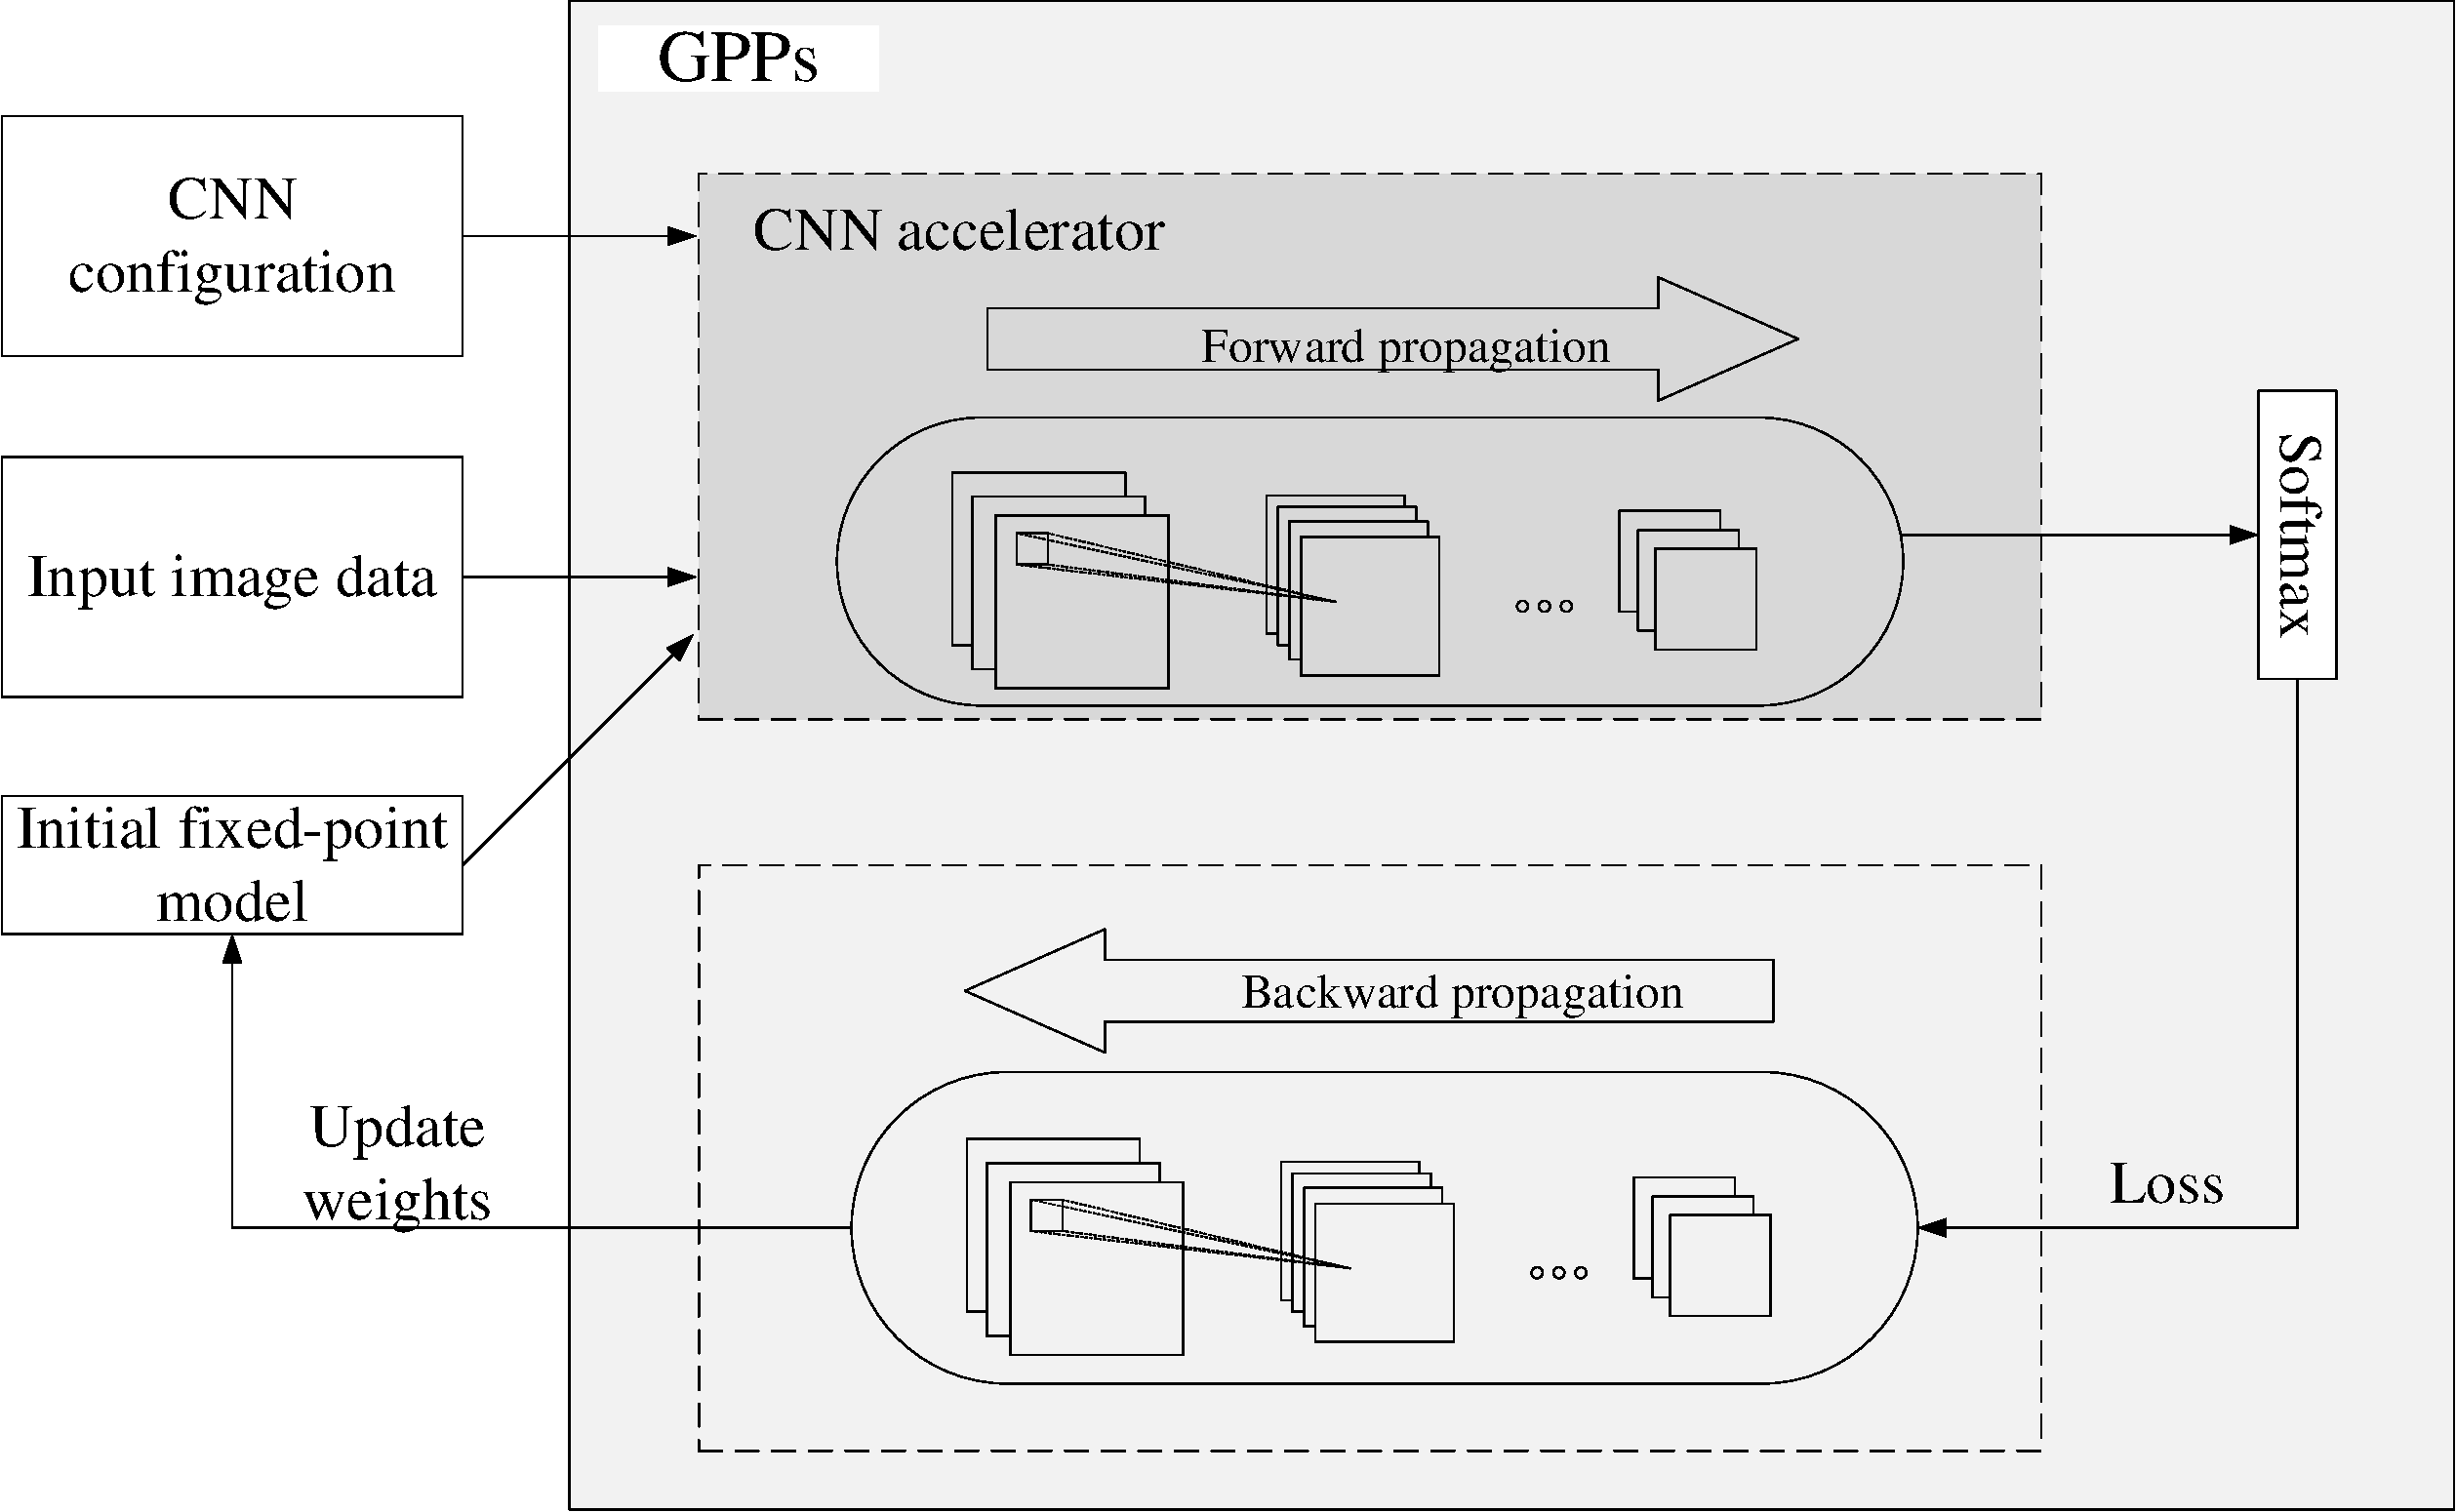
\includegraphics[width=0.95\linewidth]{retrain_framework}}
    \caption{On-accelerator neural network retraining framework.}
\label{fig:retrain}
\vspace{-1em}
\end{figure}

In this work, we utilized an OpenCL based CNN accelerator. The communication between 
host and the accelerator can be conveniently achieved with the OpenCL API. 
Many RTL based CNN accelerators can also be wrapped up with 
OpenCL API and reuse the retraining framework with minor modification.
Similar platform can also be found in \cite{Caffeine_6} and \cite{DiCecco_4}.

\subsubsection{Overclocked CNN accelerator with severe accuracy loss}
When the accuracy loss gets too large, it indicates low-probability severe timing 
violations occur on the CNN accelerators. The basic idea is to repeat the execution. 
However, when the errors are detected, previous computing results may already suffer 
the errors and the results can already be wrong. To address this problem, we opt to 
utilize the checkpoint strategy to recover from previous checkpoint. 
Fig \ref{fig:loss_checkpoint} shows the basic control flow of the checkpoint strategy.
Basically, we divide the input data stream into blocks and a set of golden reference data 
will be added to the end of each block. With the reference data, neural network accuracy 
can be measured and used for accuracy loss estimation. Then the runtime manager 
can decide the processing with the estimation. When the accuracy loss is acceptable, 
the processing will continue. When the accuracy loss is too large, the processing 
will roll back to the checkpoint. The runtime manger will be detailed 
in the next subsection. 

\begin{figure}
	\center{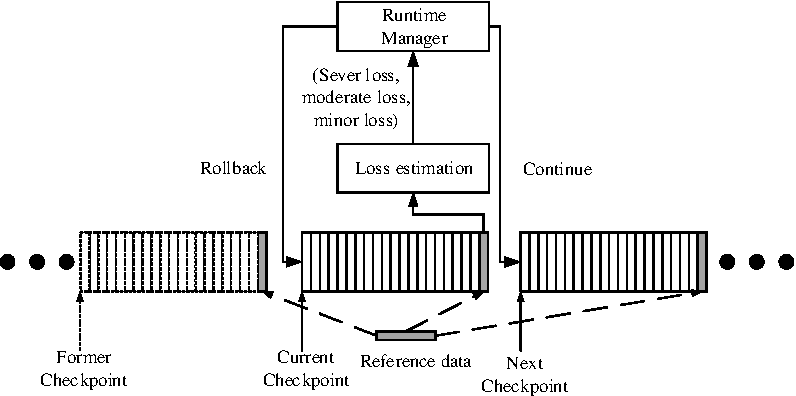
\includegraphics[width=0.95\linewidth]{loss_checkpoint}}
    \caption{Runtime checkpoint strategy.}
\label{fig:loss_checkpoint}
\vspace{-1em}
\end{figure}

\subsubsection{Runtime overclocking management}
As discussed in the above section, the accelerator status may transit at runtime, 
while corresponding remedies will be applied in different situations. To bridge the 
gap, we propose a runtime overclocking management strategy as shown in 
Fig \ref{fig:runtime-management} to handle all the possible overclocking problems 
at runtime automatically.

\begin{figure}
	\center{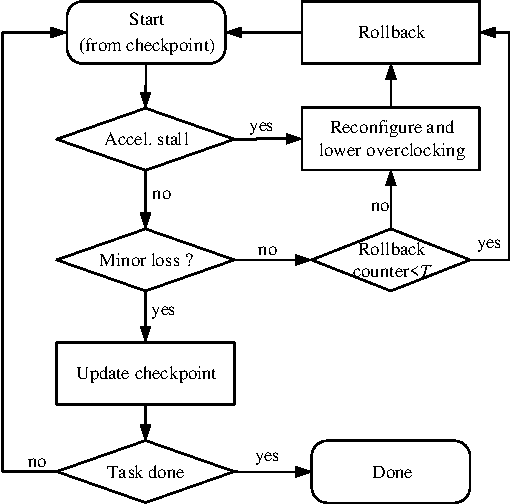
\includegraphics[width=0.75\linewidth]{manegment}}
    \caption{Runtime overclocking management.}
\label{fig:runtime-management}
\vspace{-1em}
\end{figure}

When the overclocked CNN accelerator is applied for inference, 
a watch-dog must be enabled to detect if the accelerator is stalled 
at runtime. When the accelerator is stalled, it indicates that critical 
signals are corrupted. The manger will invoke the reconfiguration 
and reload an implementation with lower overclocking. Meanwhile, 
it also rolls back the processing using the checkpoint strategy. 
When there is no system stall, accuracy loss will be evaluated 
with the granularity of a block or checkpoint. 
When there is just minor accuracy loss, the block execution is 
considered to be valid and the checkpoint will 
be updated. When the accuracy loss is non-trivial and there have been multiple rollbacks 
on this checkpoint, we consider the accelerator overclocking to be too aggressive.
Then we reconfigure the FPGA with a more conservative implementation 
and roll back for another execution on current checkpoint.
Note that we set a rollback counter and compare it with a threshold $T$ 
to determine if we should choose the reconfiguration route or the simple rollback route.
This scheme is used to avoid lowering clock when the accuracy loss is 
caused by a transient error.



